\documentclass{article}

\makeatletter
\renewcommand*{\fps@figure}{!htb}
\renewcommand*{\fps@table}{!htb}
\makeatother

\usepackage{geometry}
 \geometry{
 a4paper,
 total={170mm,257mm},
 left=20mm,
 top=20mm,
 }
 \usepackage[utf8]{inputenc}
\usepackage[hidelinks]{hyperref}
\usepackage{amsmath, bm}
\DeclareMathOperator*{\argmax}{arg\,max}
\DeclareMathOperator*{\argmin}{arg\,min}

\usepackage[ruled,vlined]{algorithm2e}
\usepackage[capitalise, nameinlink]{cleveref}
\usepackage{amssymb}
\usepackage{graphicx}
\usepackage{float}
\usepackage{booktabs}
\usepackage[parfill]{parskip}
\usepackage{comment}
\usepackage{subcaption}

\usepackage[ruled,vlined]{algorithm2e}
\SetKwInput{KwInput}{Input}                % Set the Input
\SetKwInput{KwOutput}{Output}              % set the Output


\usepackage[sorting=none]{biblatex}
\addbibresource{report_4.bib}

\usepackage{titling}
\setlength{\droptitle}{-3cm}

\title{COMP6247 Final Assignment: Learning Controller}
\author{Wei Chien Teoh (Eugene)\\\bigskip \href{mailto:wct1c16@soton.ac.uk}{wct1c16@soton.ac.uk}}
\date{4 June 2021}

\begin{document}

\maketitle

\section{Introduction}

This report presents the findings and results for the final assignment of COMP6247~\cite{mahesanniranjanCOMP6247202021}. The code implementation is stored in a Github repository \cite{teohEugeneteohCOMP6247ReinforcementOnlineLearning2021}.

\section{Radial Basis Functions} \label{sec:rbf}

In this section, we explore the use of Radial Basis Functions (RBF) on Reinforcement and Online Learning problems.

First, RBF is used to solve a non-linear regression problem. The Airfoil Self-noise Dataset~\cite{UCIMachineLearning} from the UCI repository of machine learning is used as the problem of interest for regression. The dataset consists of samples of aerodynamic and acoustic tests of airfoil blades conducted in a wind tunnel. The features given include:
\begin{enumerate}
    \item Frequency, in Hertz
    \item Angle of attack, in degrees
    \item Chord length, in meters
    \item Free-stream velocity, in metres per second
    \item Suction side displacement thickness, in metres
\end{enumerate}
The output to be predicted is the scaled sound pressure level, in decibels.

% TODO: Mention the RBF parameters, number of centroids, sigma etc and explore how it affects the output results
% TODO: Use test set
First, we attempt to solve the problem with a linear regression in closed form, $\pmb{W} = (X^T X)^{-1} X^T \pmb{y}$. We then proceed to apply an RBF kernel with Gaussian function. Three approaches were used to solve for the RBF regression parameters:
\begin{itemize}
    \item Closed form, $\pmb{W} = (U^T U)^{-1} U^T \pmb{y}$
    \item Gradient Descent (GD), epochs = 50000
    \item Mini-batch Stochastic Gradient Descent (SGD), batch size = 64, epochs = 10000
\end{itemize}
The Mean Squared Error (MSE) results are shown in \cref{tab:mse-regression}. Linear regression is shown to be insufficient in solving this problem, as the MSE calculated is substantially higher than RBF regression solutions. The RBF closed-form solution provided the optimal solution. Both gradient descent methods show convergence of the loss function and also provided similar results, as illustrated in \cref{fig:gd-loss}. Also SGD shows more fluctuations during the training, it requires fewer number of epochs before convergence. The loss of the gradient descent methods can be further optimised by lowering the learning rate or using adaptive methods.

\begin{table}
    \centering
    \caption{Mean squared error for regression problem.}
    \label{tab:mse-regression}
    \begin{tabular}{lr}
    \toprule
    Model &         MSE \\
    \midrule
    Linear          &  915.288358 \\
    RBF Closed Form &   33.754672 \\
    RBF GD          &   49.234992 \\
    RBF SGD         &   48.822703 \\
    \bottomrule
    \end{tabular}
\end{table}

\begin{figure}
    \centering
    \begin{subfigure}{.49\linewidth}
        \centering
        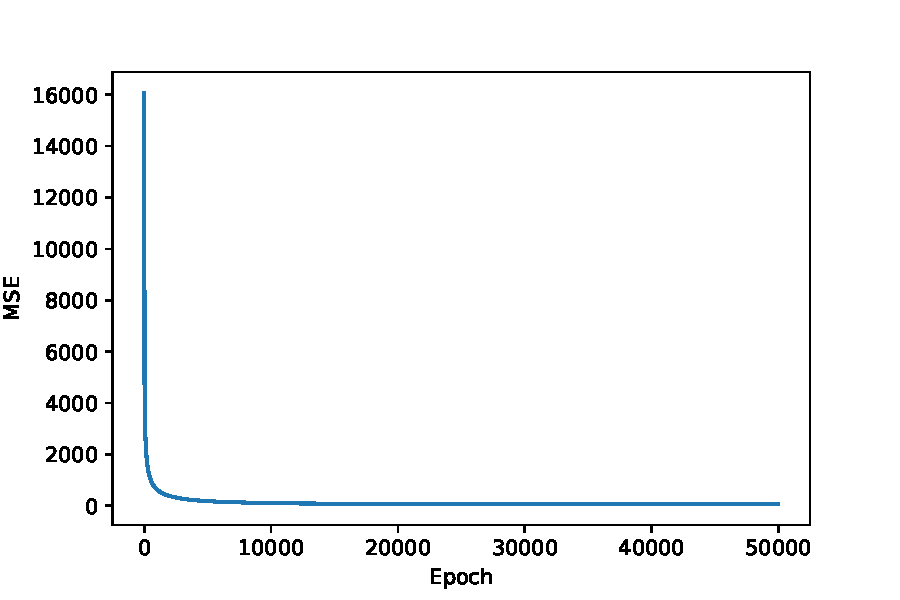
\includegraphics[width=\linewidth]{Figures/gd-loss.pdf}
        \caption{Gradient Descent}
    \end{subfigure}
    \begin{subfigure}{.49\linewidth}
        \centering
        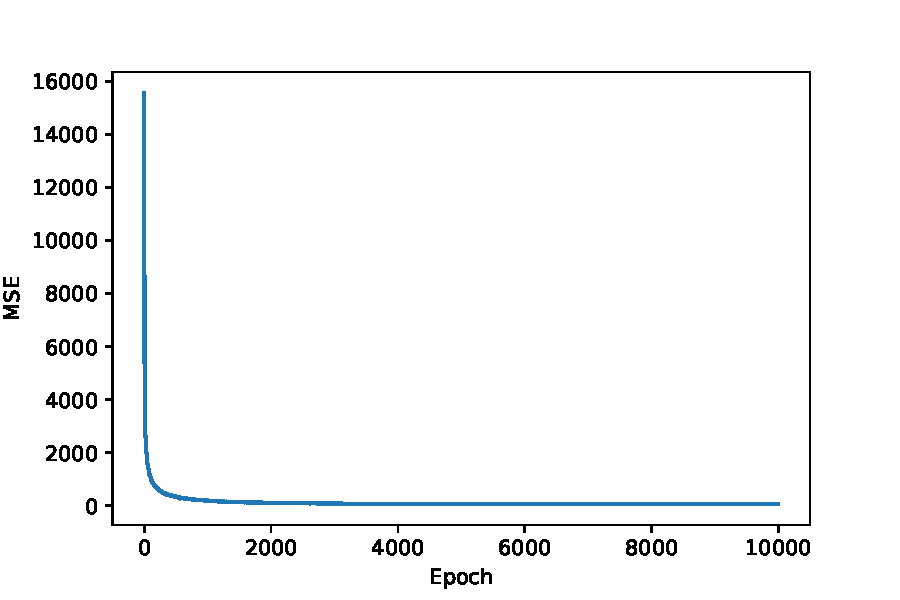
\includegraphics[width=\linewidth]{Figures/sgd-loss.pdf}
        \caption{Stochastic Gradient Descent}
    \end{subfigure}
    \caption{Log-scaled loss curves for regression using gradient descent approaches.}
    \label{fig:gd-loss}
\end{figure}

\section{Mountain Car Learning Controller}

In this section, we explore the mountain car problem~\cite{mooreEfficientMemorybasedLearning1990}. More specifically, we will attempt to learn a controller for the car to drive up a steep hill. We will explore several Temporal Difference (TD) learning algorithms and investigate the performance of them.

\subsection{Tabular Q Learning}

Learning a controller involves learning an optimal policy. In Q learning, the action-value function is learned instead. The optimal policy and its associated value function can be further derived as:

\begin{equation}
    \begin{split}
        \pi^* &= \argmax_{a} Q(s, a) \\
        V^* &= \max_{a} Q(s, a) 
    \end{split}
    \label{eq:optimal-V}
\end{equation}

The mountain car problem can be discretised into grids, where each block of the grid describes a state of which the car/agent is present. In this experiment, the problem is discretised into 40 states per state dimension (position and velocity). The Q function is tabularised with a dimension of $\mathbb{R}^{40 \times 40 \times 3}$, of which there exist $40 \times 40$ states and 3 actions, $a \in {-1, 0, 1}$ (left, neutral, right). The algorithm is performed for 1000 episodes, where the episode length is illustrated in \cref{fig:ep-length}. Note that the reward is described as -1 for every time step, thus the episode length can also be interpreted as the negative reward. For all experiments in this report, the $\epsilon$-greedy policy will be used during training, where $\epsilon$ is set to 0.05. The plot shows evidence of the convergence towards an optimal policy which maximises reward, synonymous to minimising episode length.

\begin{figure}
    \centering
    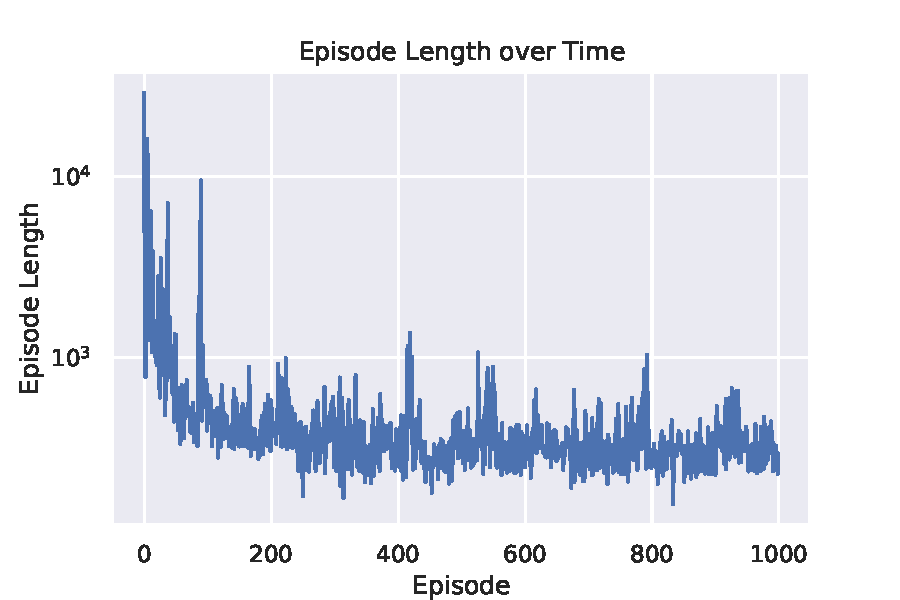
\includegraphics[width=.7\linewidth]{Figures/ep_length.pdf}
    \caption{Log-scaled episode length over time. Final episode length = 154.}
    \label{fig:ep-length}
\end{figure}

Following \cref{eq:optimal-V}, the optimal value function can be obtained by taking the maximum of the corresponding action with maximises the reward.

% TODO: explain how to obtain X
After obtaining the optimal value function, we attempt to approximate it using RBF regressors previously explored in \cref{sec:rbf}. However, an RBF sampler using the Random Kitchen Sink~\cite{rahimiRandomFeaturesLargeScale} algorithm will be used as an approximation to the RBF kernel. The RBF sampler approximates the RBF by using Monte Carlo random sampling of its Fourier transform. The number of basis functions, $J$ is varied and the centroids are randomly initialised. The scaling factor, $\sigma_j$ is set to $1.0$. Scaling does not provide significant effects to the results and thus is not further explored. Note that setting a global $\sigma_j$ will allow the RBF network to have universal approximation capability~\cite{wuUsingRadialBasis2012}. The RBF regressors are solved using the closed form solution.

% explain how to get approximated value function from approximated action-value function
% can be re-written/improved
\cref{fig:value-functions} shows both the true and several examples of approximated value functions with different basis functions. Lesser number of RBF basis functions causes the approximated value function landscape to be less refined, whereas greater number of basis functions produce landscapes which are visually different from the true landscape. The optimal approximation using RBF regression is with 20 basis functions, with an average reward of -128.4 and an MSE of 59 compared to the true value function. The approximated action-value functions are further reused as the optimal policy for the mountain car environment, of which the episode lengths are evaluated. The episode lengths and the MSE illustrated in \cref{fig:metrics-rbf} is shown to reflect the phenomenon shown in the value function landscapes. The episode length of lesser than 5 and greater than 25 basis functions does not converge even after 5000 steps. However, there are selected few (around 41 basis functions) that still provide good performances relative to the optimal value function (20 basis functions). The anomaly is potentially due to it's basis functions having similar shape to the true value function, even when it's MSE is shown to exponentially diverge from the true value function after 25 basis functions, illustrated in \cref{fig:mse-j}.


\begin{figure}
    \centering
    \begin{subfigure}{.49\linewidth}
        \centering
        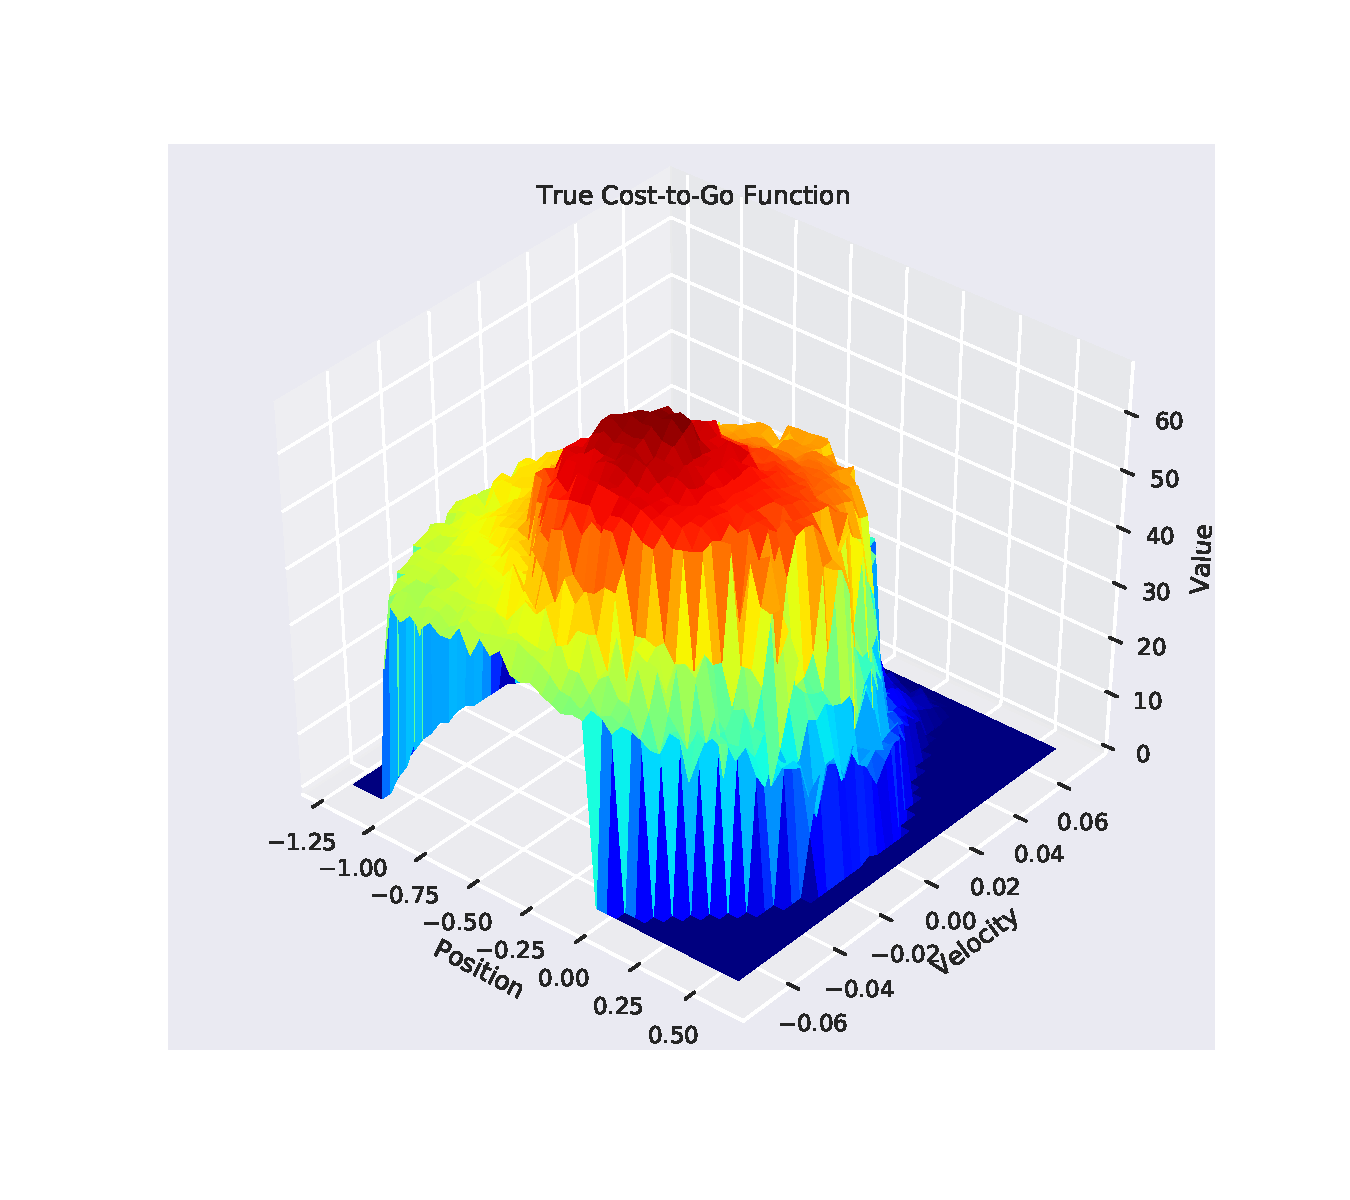
\includegraphics[width=\linewidth]{Figures/true_value_function.pdf}
    \end{subfigure}
    \begin{subfigure}{.49\linewidth}
        \centering
        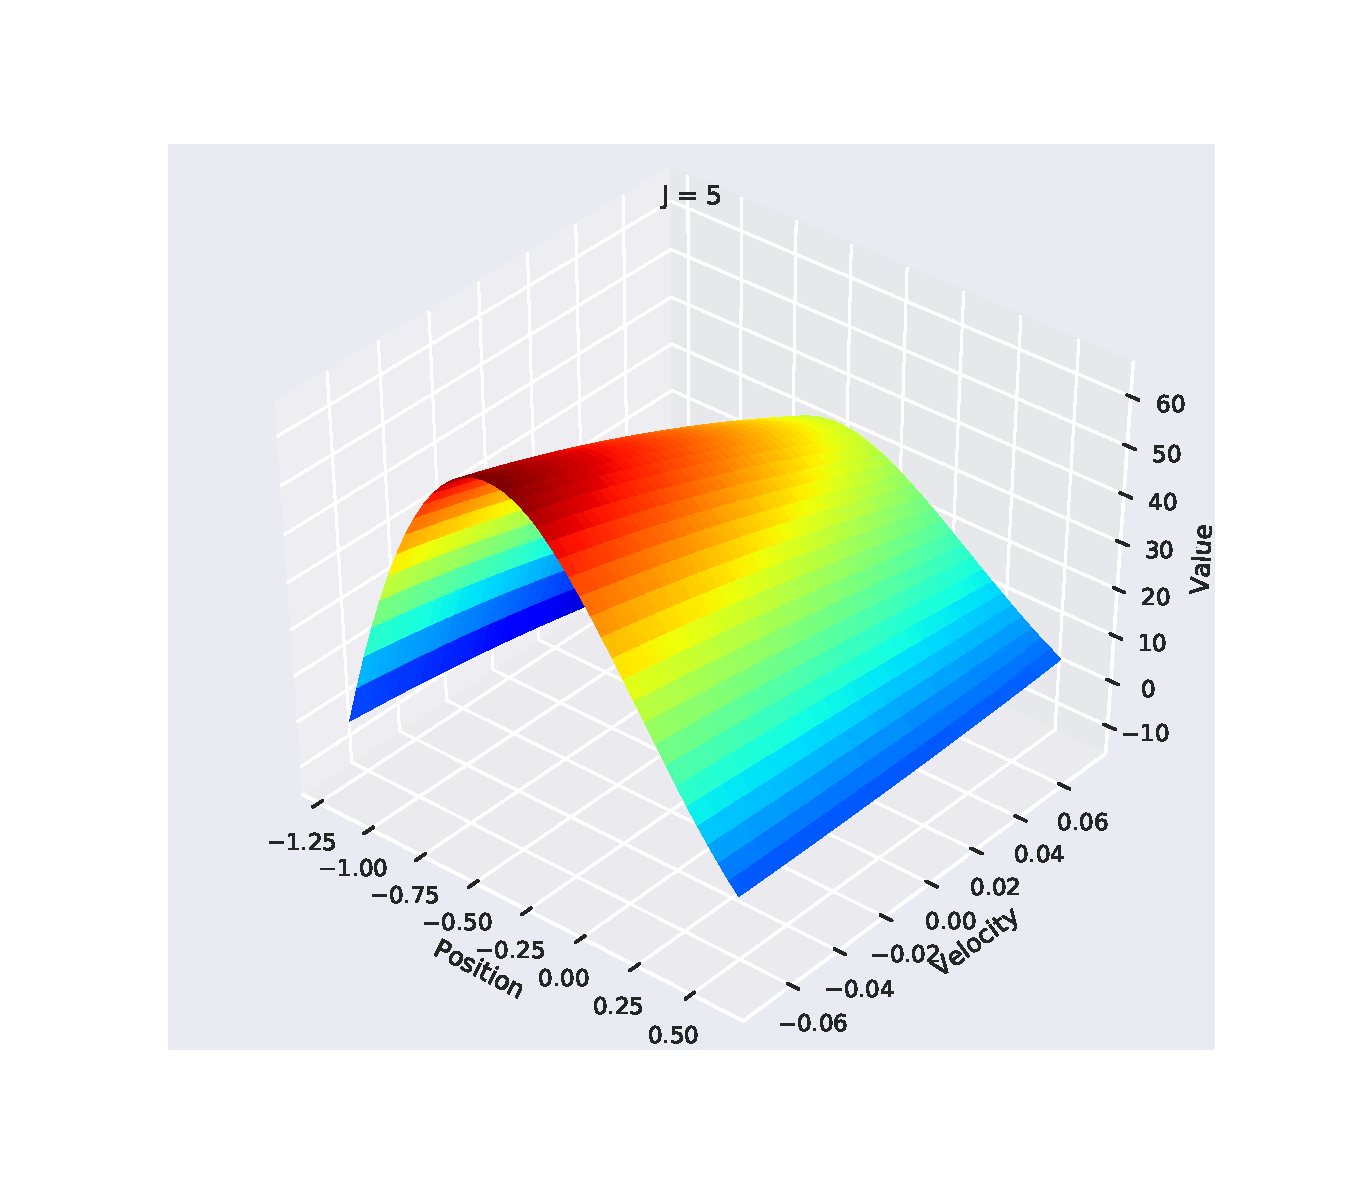
\includegraphics[width=\linewidth]{Figures/rbf_value_function_5.pdf}
    \end{subfigure}

    \begin{subfigure}{.49\linewidth}
        \centering
        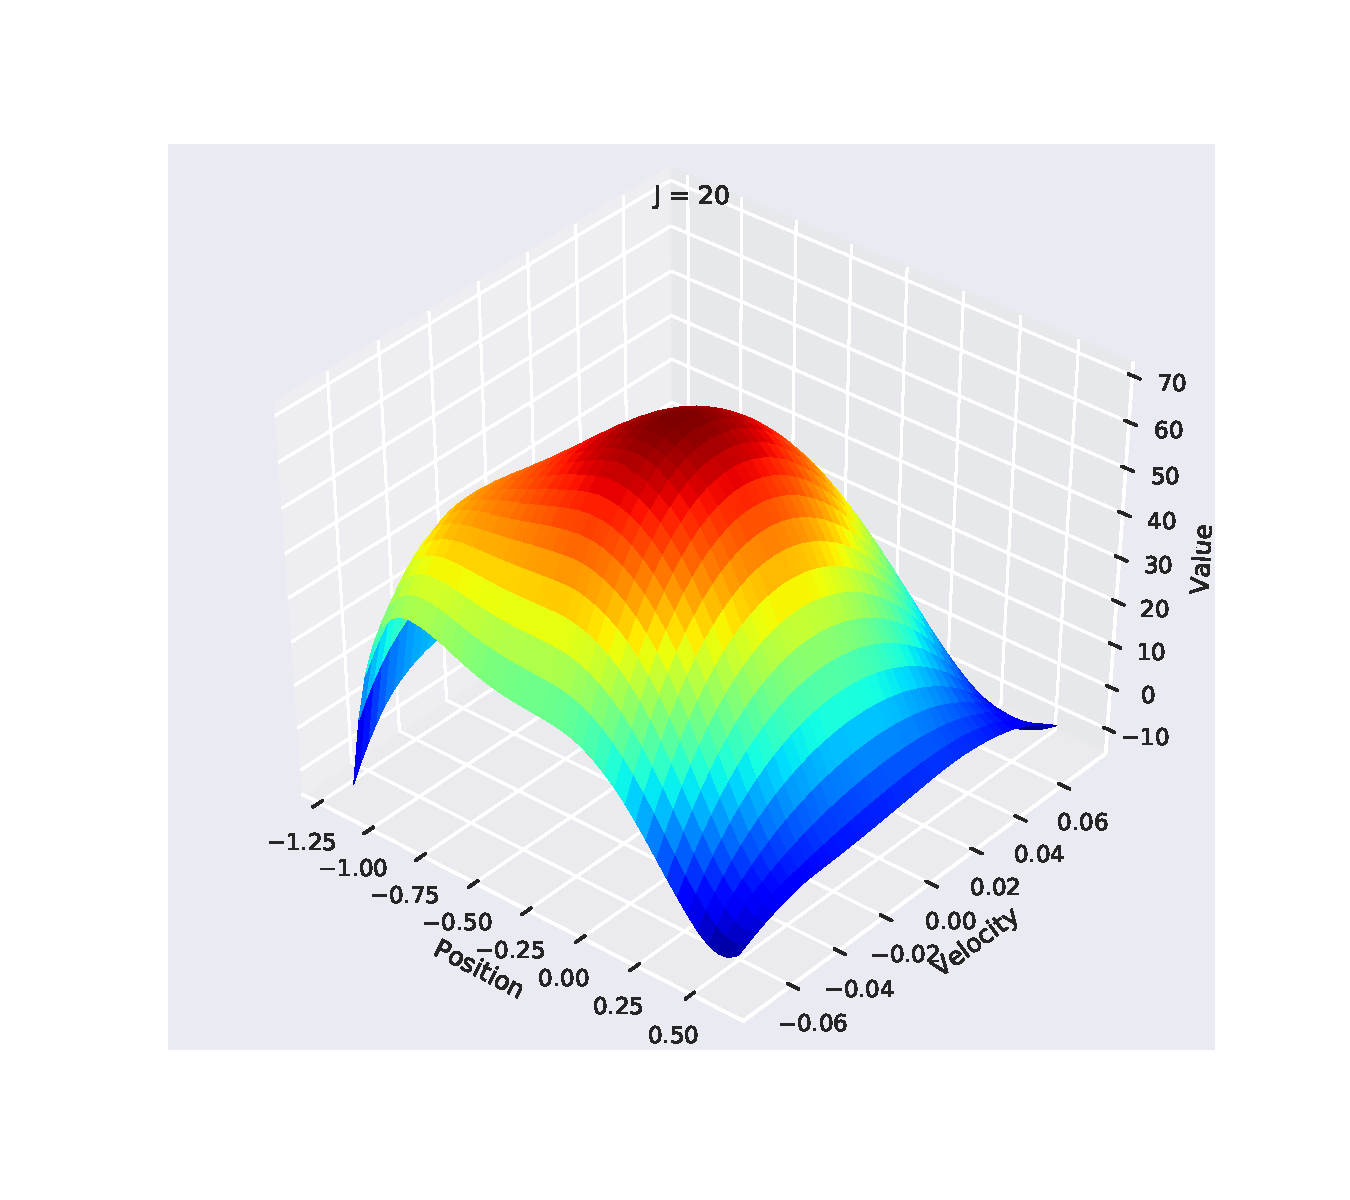
\includegraphics[width=\linewidth]{Figures/rbf_value_function_20.pdf}
    \end{subfigure}
    \begin{subfigure}{.49\linewidth}
        \centering
        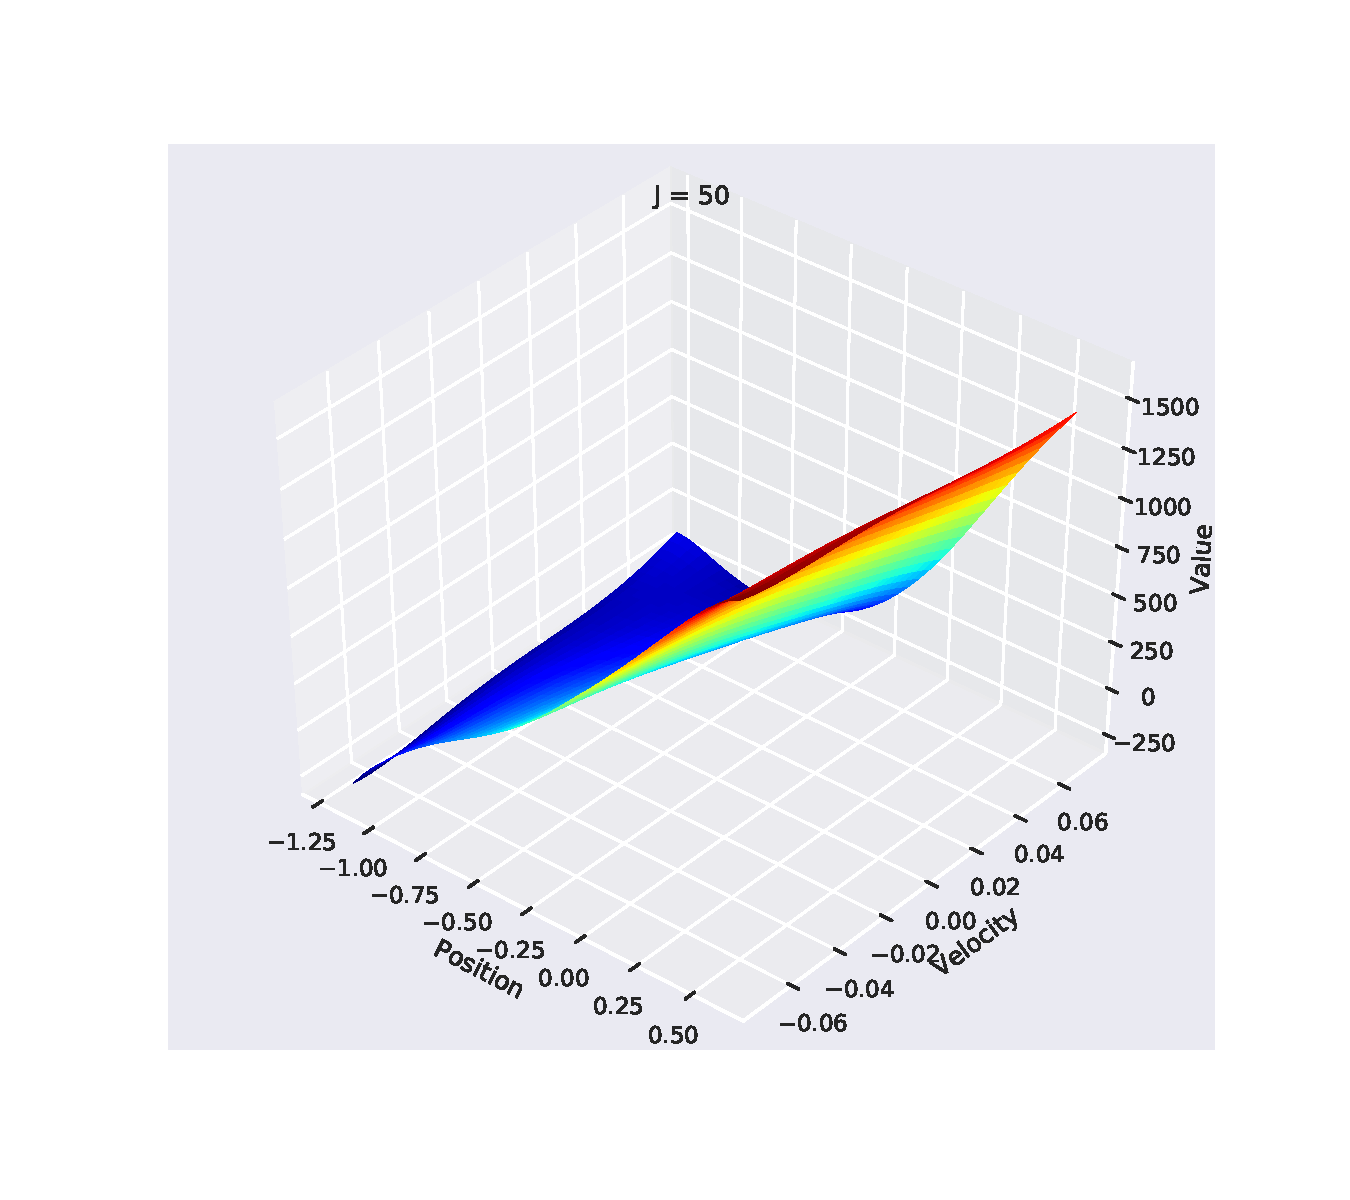
\includegraphics[width=\linewidth]{Figures/rbf_value_function_50.pdf}
    \end{subfigure}
    \caption{Cost-to-Go functions. (Top left) True value function. (Others) RBF approximation of value function with different number of basis functions, $J$.}
    \label{fig:value-functions}
\end{figure}

\begin{figure}
    \centering
    \begin{subfigure}{.49\linewidth}
        \centering
        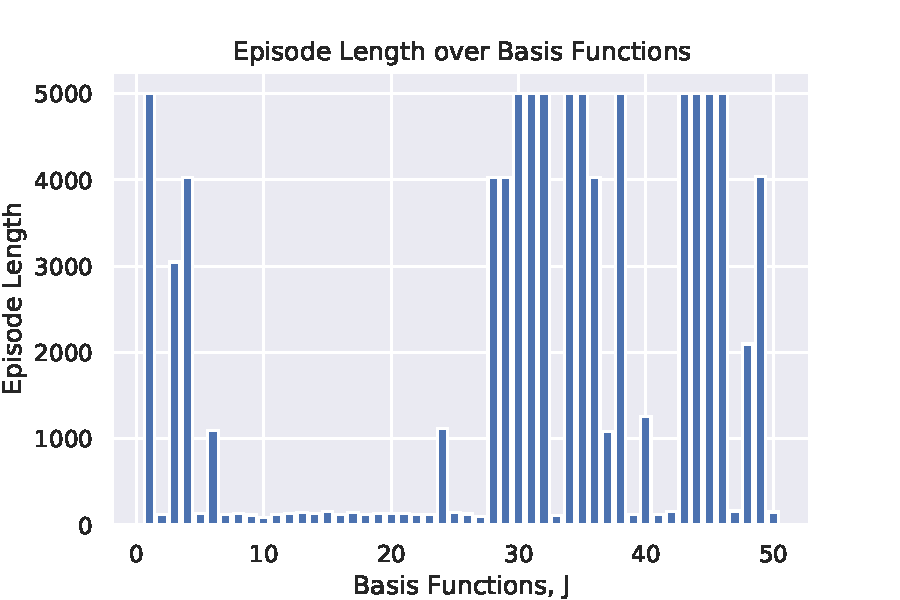
\includegraphics[width=\linewidth]{Figures/ep_steps_j.pdf}
        \caption{Episode length over number of basis functions, averaged over 5 runs. The environment is terminated after 5000 steps.}
        \label{fig:ep-steps-j}
    \end{subfigure}
    \begin{subfigure}{.49\linewidth}
        \centering
        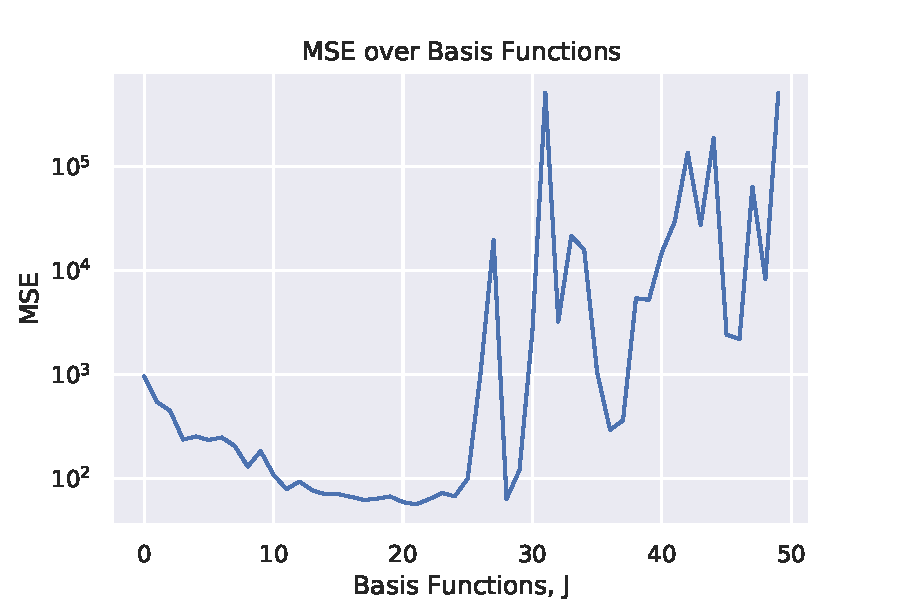
\includegraphics[width=\linewidth]{Figures/mse_j.pdf}
        \caption{Log-scaled MSE over number of basis functions.}
        \label{fig:mse-j}
    \end{subfigure}
    \caption{Relevant metrics over different number of basis functions.}
    \label{fig:metrics-rbf}
\end{figure}

\subsection{TD Learning with Function Approximation}

We previously attempted to solve the mountain car problem by tabular discretisation of Q Learning. We then explored the use of RBF Networks to approximate the tabular Q function. One could combine these two concepts by directly learning the weights of the function approximator using online learning methods such as stochastic gradient or bayesian inference. In this section, we will explore both on-policy and off-policy Temporal Difference learning methods, namely Q Learning and SARSA, of which the Q function will be approximated by RBF networks.

\begin{equation}
    Q(s, a) \approx \hat{q}(s, a) = \sum_{j = 1}^{J} w_j \phi(\Vert \pmb{x} - \pmb{m}_j \Vert / \pmb{\sigma}_j)
\end{equation}

There are several advantages to function approximation of the Q function:
\begin{itemize}
    \item As the number of state spaces become large, it is infeasible to tabulate values of each state space due to computational constraints. This also applies to continuous state space.
    \item Function approximation allows generalisation to unseen state spaces. Hence, it is not needed to explore every possible state to obtain an optimal policy or value function.
    \item Raw and unstructured data such as images can be directly be fed into the function approximator using state-of-the-art approaches such as Convolutional Neural Networks.
\end{itemize}

There are several approaches to the parameterization of the function approximator. Since Q takes both the states and actions as inputs, one could build a regressor for each action. However, it requires linear time to obtain the max or argmax of the action values. Alternatively, the RBF can be represented as a shallow neural network with multiple output nodes for each action \cite{mnihPlayingAtariDeep2013}. Computing the max or argmax would then only result in taking the maximum value of the outputs. Since it is a neural network, the weights, centres, and scaling parameters can also be learned through backpropagation. Both the neural network and the backpropagation approaches were attempted, but was unable to obtain a stable convergence of the Q function. This is potentially due to the large number of learnable parameters (including centres and scaling) and the stochasticity of the gradients in comparison to the small number of states and actions. Thus, the original linear time approach will be used in this experiment.

Again, the RBF kernel was approximated using the Random Kitchen Sink algorithm with $\sigma_j$ as $1.0$. As before, $\sigma_j$ will not be tuned or modified in the experiments, as the objective in this section is to attempt to successfully utilise function approximation to further improve on previous methods. Three regressors were built for each action. The regressors were trained for 500 episodes. It should be noted that it required more time, approximately 4 times on average to train the function approximators. Five different number of basis functions, $J = (5, 10, 15, 20, 50)$ was used, and finally the one with maximum reward is selected and illustrated in \cref{fig:func_approx}. Both plots did not achieve approximations as well as those in \cref{fig:value-functions}. This is potentially due to the stochasticity and the insufficient episodes due to time constraints. The stochasticity is caused by updating the gradient descent only one sample at a time. \emph{Experience replay} can be introduced to solve this, where the experiences at each time step, $e_t = (s_t, a_t, r_t, s_{t+1})$ is stored over many episodes to perform mini-batch updates of gradient descent. In spite of the approximations, both Q Learning and SARSA with function approximation provided comparative rewards to the tabular method.

% TODO: Talk about Q Learning vs SARSA
% TODO: Add episode length plot

From the discussion and analysis above, it can be concluded that both tabular and function approximation approaches to TD learning were able to successfully solve the mountain car problem in with descent rewards. As the scale of the problem is small, the tabular discretisation method is proven to be the better choice, exceeding the function approximation method in the number of hyperparameters to tune,training time and expected reward.

\begin{figure}
    \centering
    \begin{subfigure}{.49\linewidth}
        \centering
        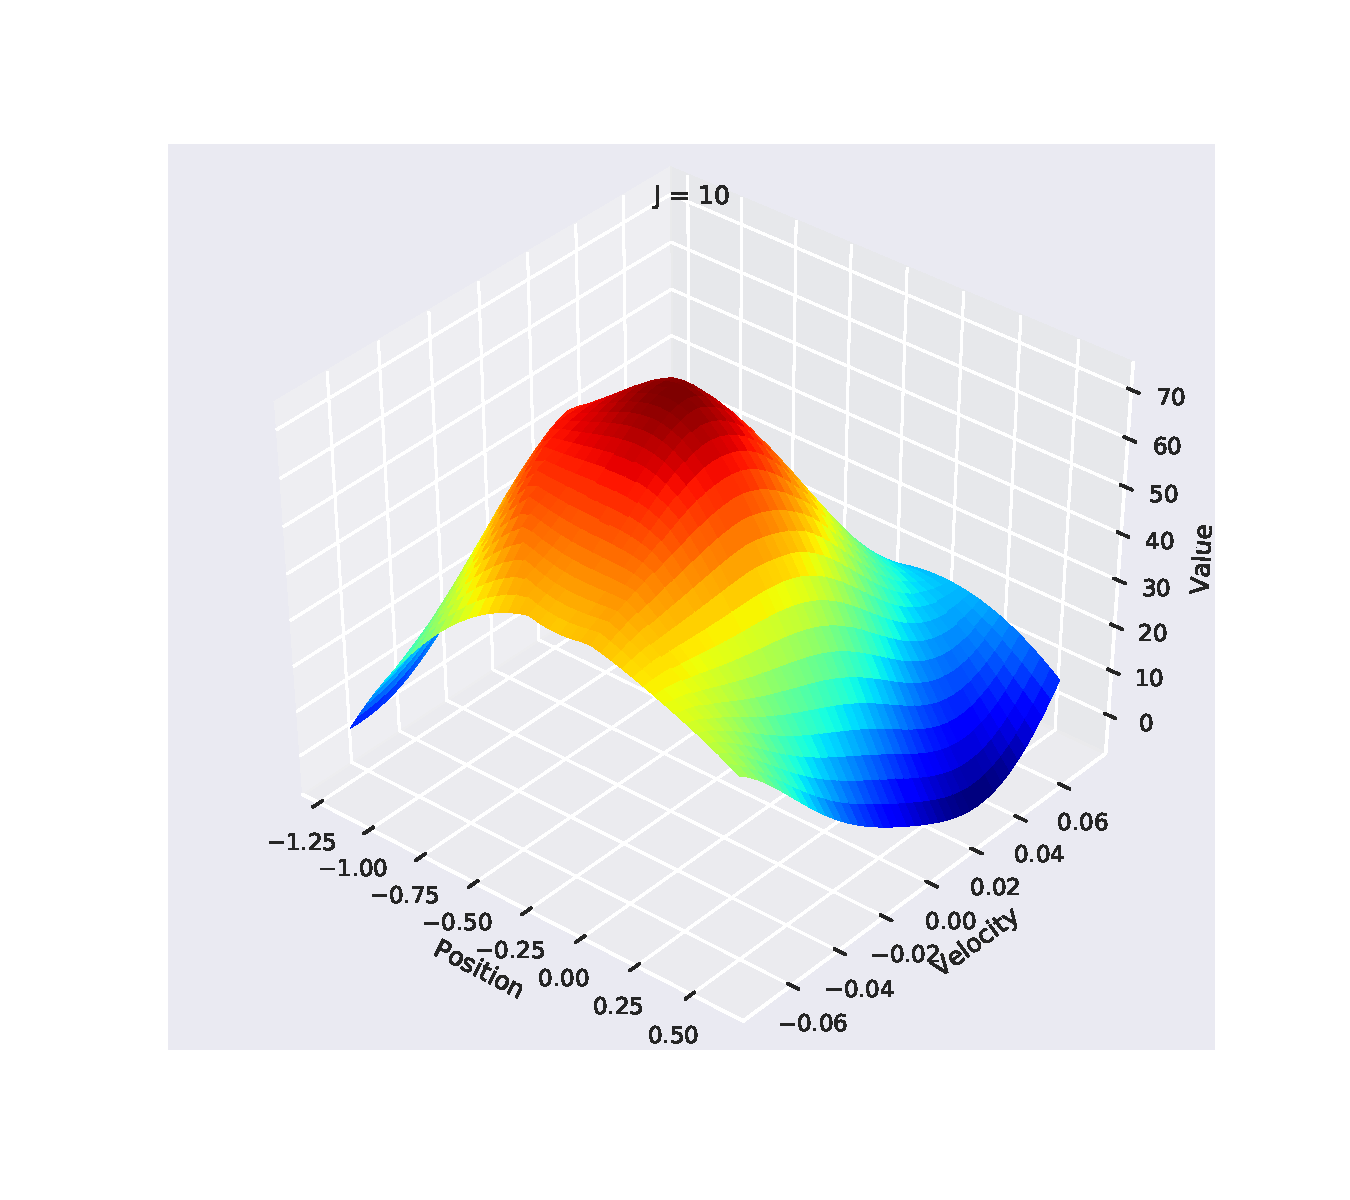
\includegraphics[width=\linewidth]{Figures/func_approx_q_learning_value_func_10.pdf}
        \caption{(Q Learning) Average reward: -162.2 \\ MSE: 245.1}
        \label{fig:q_learning}
    \end{subfigure}
    \begin{subfigure}{.49\linewidth}
        \centering
        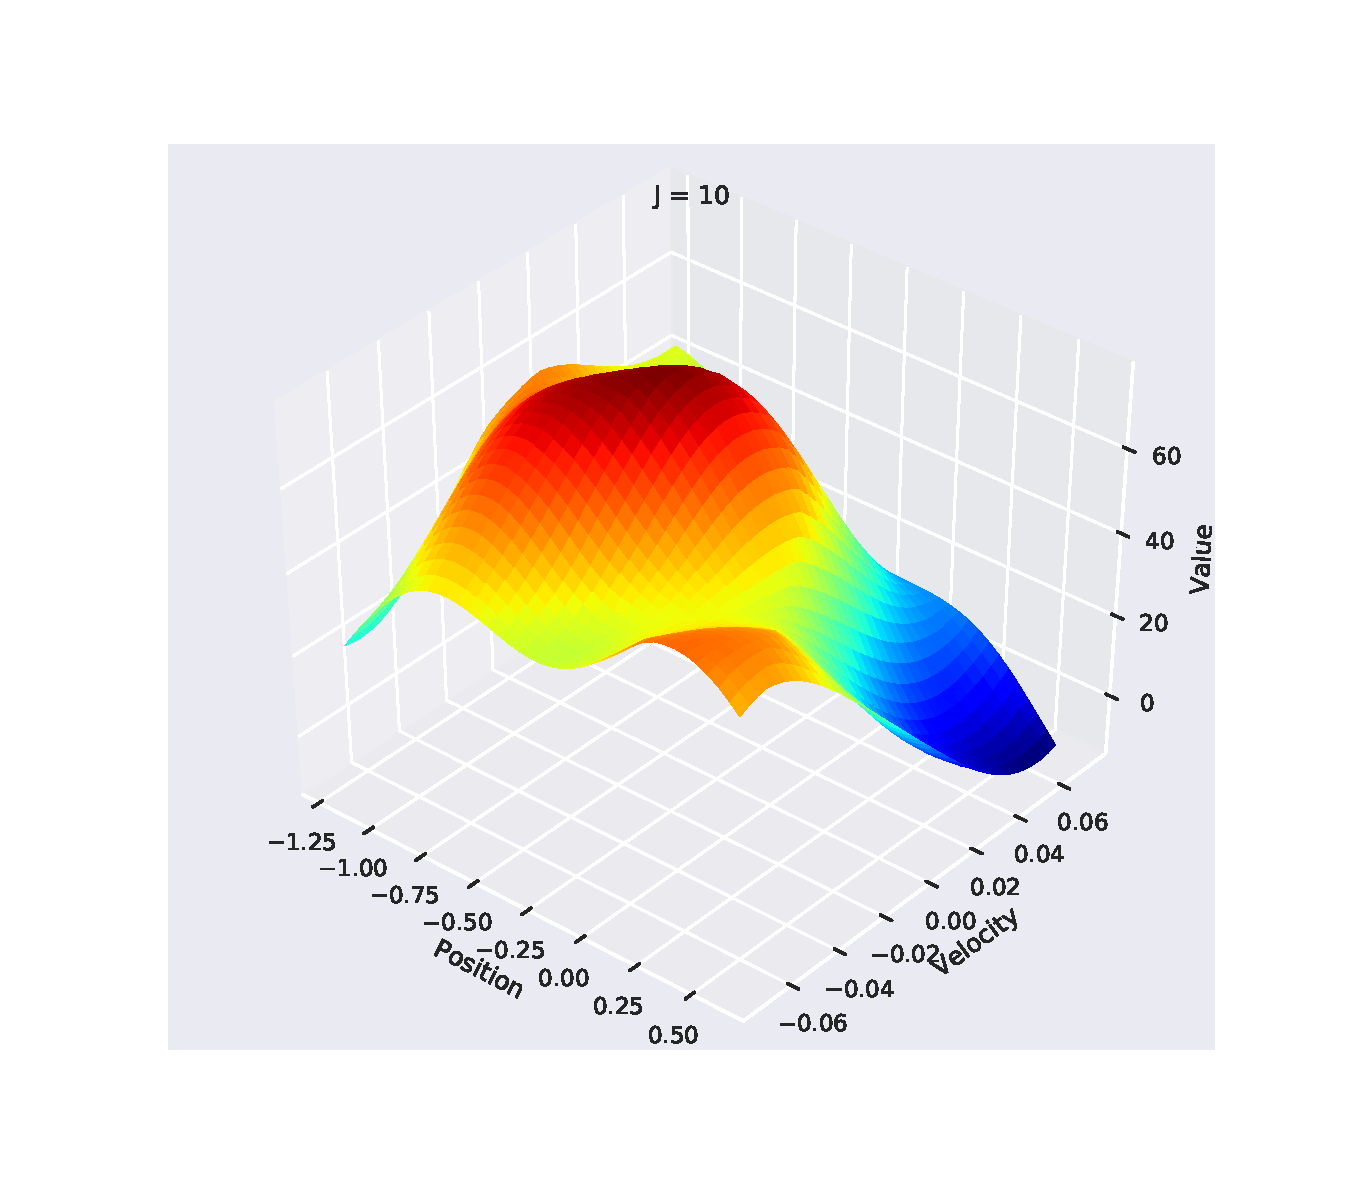
\includegraphics[width=\linewidth]{Figures/func_approx_sarsa_value_func_10.pdf} 
        \caption{(SARSA) Average reward: -167.2 \\ MSE: 590.2}
        \label{fig:sarsa}
    \end{subfigure}
    \caption{Optimal Approximated Cost-to-Go Function. Optimal policy was performed for 5 runs, with average rewards stated above. MSE against the true value function is also stated.}
    \label{fig:func_approx}
\end{figure}

\subsection{Resource-Allocating Network}

In previous sections, the number of basis functions, $J$ was arbitrarily tuned by sweeping multiple different values. Such tuning method is often impractical due to the large amount of time required. A Resource-Allocating Network~\cite{plattResourceallocatingNetworkFunction1991} (RAN) allow the RBF network to grow in it's number of basis functions in an online setting, using stochastic gradient descent. RAN is able to find the optimal number of basis functions by learning from the presented data. RAN grows its network by considering two conditions:

\begin{equation}
    \begin{split}
        \Vert \pmb{x}_n - \pmb{u}_{nr} \Vert > \zeta_n\\
        e_n = y_n - f(\pmb{x}_n) > e_{\min}\\
    \end{split}
\end{equation}

where:
\begin{itemize}
    \item an observation $(\pmb{x}_n, y_n)$ is given
    \item $\zeta_n = \max(\zeta_{\max} \gamma^n, \zeta_{\min})$
    \item $\pmb{u}_{nr}$ is the nearest centroid to $\pmb{x}_n$
\end{itemize}


Such approach can be extended to TD learning methods, where RAN can be combined with function approximation. An example of Q learning with RAN is shown in \cref{algo:ran}. The algorithm can also be modified to work with SARSA by changing the TD error to using the same policy (e.g. $\epsilon$-greedy).

\begin{algorithm}[htb!]
    \SetAlgoLined
    \DontPrintSemicolon
    \KwInput{step size $\eta \in (0, 1]$, small $\epsilon > 0$, $\zeta_{\min} > 0$, $e_{\min} > 0$, $\zeta_{\max} > e_{\min}$, $0 < \gamma > 1$}
    $\hat{q}(s, a, \pmb{w}) = w_0 + \sum_{j=1}^{J} w_j \phi_j(s, a)$, where $\phi(s, a)$ is an RBF kernel with centroid $u_j$ and scaling factor $\sigma_j$\;
    Initialize weights $\pmb{w}$ arbitrarily (e.g., $\pmb{w} = \pmb{0}$)\;
    $\zeta_n$ = $\zeta_{\max}$, $w_0 = y_0$\;
    \For{each episode}{
        $S, A \leftarrow$ initial state and action of episode (e.g. $\epsilon$-greedy)\;
        \For{each step of episode} {
            \tcc{TD error}
            Take action $A$, observe $R, S'$\;
            $\zeta_n = \max(\zeta_{\max} \gamma^n, \zeta_{\min})$\;
            \If{$S'$ is terminal} {
                $e_n = R - \hat{q}(S, A, \pmb{w}^{(n)})$\;
            } \Else {
                $e_n = R + \argmax_a \hat{q}(S', a, \pmb{w}^{(n)}) - \hat{q}(S, A, \pmb{w}^{(n)})$\;
            }
            \If{$e_n > e_{\min}$ and $\Vert \pmb{x}_n - \pmb{u}_{nr} \Vert > \zeta_n$}{
                \tcc{Allocate a new hidden unit}
                $\alpha_{K+1} = e_n$\;
                $\pmb{u}_{K+1} = \pmb{w}_n$\;
                $\sigma_{K+1} = \kappa \Vert \pmb{w}_n - \pmb{u}_{nr} \Vert$\;
            } \Else {
                $\pmb{w}^{(n+1)} = \pmb{w}^{(n)} + \eta e_n \pmb{w}_n$\;
            }
            $S \leftarrow S'$\;
        }
    }
    \caption{Q Learning with RAN Function Approximation.}
    \label{algo:ran}
\end{algorithm}

Suppose the model is non-linear, which an RBF network is of that, one can further extended the RAN algorithm by replacing the Least Mean Squares (LMS) algorithm (or SGD) with non-linear state estimation methods. The EKF is shown to work relatively well~\cite{kadirkamanathanFunctionEstimationApproach1993}. If the model is highly non-linear, bayesian inference methods such as Sequential Importance Sampling is also feasible.

\section{Learning to Optimize Neural Nets: Review}

The paper ``Learning to Optimize Neural Nets''~\cite{liLearningOptimizeNeural2017} proposes a framework for learning optimization algorithms using reinforcement learning. Learning to optimize is a difficult problem as there exist many different types of objective functions, input data, and learning algorithms. Previous work from Bengio et al.~\cite{LearningSynapticLearning} proposed a way to learn the formula used to update the model parameters during learning. However, the learned formula does not take the objective function into account, thus generalisation is an issue. Maclaurin et al.~\cite{maclaurinGradientbasedHyperparameterOptimization2015} proposed to learn regularization hyperparameters and learning rate scheduler. However, the generalization of hyperparameters to other objective functions was not considered. More recently, Andrychowicz et al.~\cite{andrychowiczLearningLearnGradient2016} proposed a method to learn from the objective function through backpropagation on a particular task using supervised learning. Again, the method fails to generalise to unseen objective functions, thus only allowing it to be applicable in specific tasks the model is trained on. The method which this paper proposes attempts to learn to optimize task-independent objective functions. The problem can be represented as a reinforcement learning problem, where an optimal policy is learned by rewarding those that converge quickly and penalizing those that do not. It will not depend on the data it is given but rather only the environment it interacts with. The author claims this approach could solve the generalisation problem of learning to optimize.

Rather than maximizing over rewards, the optimal policy to be will be minimizing the expectation over a sequence of states and actions of the summation of the cost $c$. The cost in this case is the true objective value $f(x^{(t)})$. 

\begin{equation}
    \pi^{*} = \argmin_{\pi} \mathbb{E}_{s_0, a_0, s_1, \cdots, s_T} [\sum_{t=0}^{T} c(s_t)]
    \label{eq:optimal-policy}
\end{equation}

In \cref{eq:optimal-policy}, there involves an expectation value of a joint distribution over states and actions. Expectations typically involve integrals, which are often intractable. The author then proposed the use of function approximators to approximate 
$\pi (a_t | o_t, t) = \mathbb{N} (\mu^{\pi} (o_t), \Sigma^{\pi} (o_t))$, where the functions $\mu^{\pi}(\cdot)$ and $\Sigma^{\pi} (\cdot)$ are learned.

The state $s_t$ include:
\begin{itemize}
    \item $x^{(t)}$, the current iteration loss
    \item $\phi(x^{(1)}, \cdots, x^{(t)})$, features depending on the previous iterations
    \item $\nabla \hat{f}(x^{(1)}), \cdots, \nabla \hat{f}(x^{(t)})$, gradients
    \item $\hat{f}(x^{(1)}), \cdots, \hat{f}(x^{(t)})$, values from the objective function
\end{itemize}

The action $a_t$ is the update to the iteration $\Delta x$.

With the optimization problem defined above, it can then be solved with any reinforcement learning algorithm which is able to obtain the optimal policy $\pi^*$. The author proposed the use of Guided Policy Search (GPS). GPS introduces a new policy, $\psi$. The algorithm performs policy optimization on $\psi$, then uses it to train $\pi$. The constrained optimization problem of GPS is defined in \cref{eq:gps}. The constraints can further be relaxed by equating it's expectations. The problem can then be solved using constrained optimization algorithms, such as ADMM.

\begin{equation}
    \begin{split}
        \min_{\theta, \eta} \mathbb{E}_{\psi} [\sum_{t=0}^{T} c(s_t)] \; \text{s.t.} \; \psi (a_t | s_t, t; \eta) = \pi (a_t | s_t; \theta) \; \forall a_t, s_t, t\\
        \implies \min_{\theta, \eta} \mathbb{E}_{\psi} [\sum_{t=0}^{T} c(s_t)] \; \text{s.t.} \; \mathbb{E}_{\psi} [a_t] =  \mathbb{E}_{\psi} [ \mathbb{E}_{\pi} [a_t | s_t ]]\; \forall t
    \end{split}
    \label{eq:gps}
\end{equation}

In the experiments, the author uses shallow neural nets to train on the MNIST dataset and then tested on TFD, CIFAR-10 and CIFAR-100. The training set only consisted of one objective function, the cross-entropy loss. The experimental results has shown to work better than existing popular optimization algorithms on both the training and test datasets, especially compared to Maclaurin et al.'s work. The author successfully showed that it scales to larger neural net architectures, noisy gradients and longer time horizons.

However, there are several caveats with the experiments. The experiments only involve datasets of images, trained and tested on only one objective function. Thus, it does not fully reflect on their claim on generalising to different objective functions and tasks. Although the author attempted on larger models, it is nowhere the scale of state-of-the-art architectures such as ResNets. Moving forward, more experiments on state-of-the-art and larger models should be included, along with different data types.

Stemming from the paper, there are several open challenges that can further improve this work. First, one can improve on the algorithm to learn the intractable expectation in \cref{eq:optimal-policy}. Current reinforcement learning methods have a high variance and are highly susceptible to vanishing and exploding gradient problems. Secondly, one can improve on the generalisation of optimization algorithm trained on low-dimensional problems to high-dimensional problems.

\printbibliography

\end{document}